% !TEX root = ../notes_template.tex

\chapter{복소미분}

이 장에서는 다음 3가지 주제를 중점적으로 다룬다.

\begin{itemize}
\item[(1)] 복소미분의 정의:
즉, $\mathbb C$의 열린 부분집합 $U$에 정의된 함수 $f:U\to\mathbb C$와
$z_0\in U$가 주어졌을 때, ``$f$가 $z_0$에서 복소미분가능하고 복소미분값은 $f'(z_0)$이다''
라는 의미에 대하여 학습한다.
\item[(2)] 코시-리만 방정식: 
$\dfrac{\partial u}{\partial x} = \dfrac{\partial v}{\partial y}$와
$\dfrac{\partial u}{\partial y} = - \dfrac{\partial v}{\partial x}$.

이 방정식은 
복소미분가능함수 $f:U\to\mathbb C$의 실수부와 허수부 $u$, $v$가
만족하는 편미분방정식이다.

\begin{figure}[!h]
\begin{center}
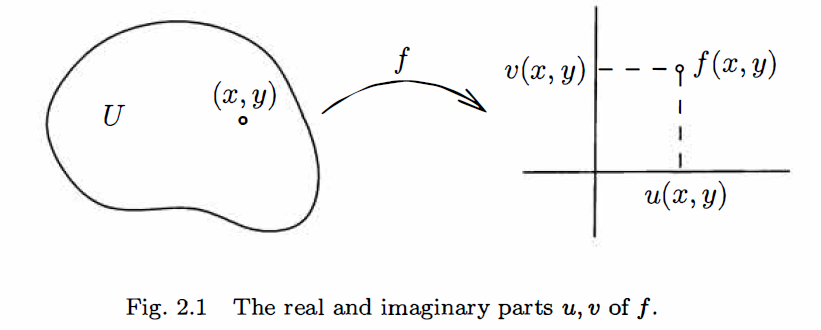
\includegraphics[width=0.6\textwidth]{./SaltChapter/fig-2-1}
\end{center}
\caption{$f$의 실수부와 허수부 $u$, $v$}
\label{fig-2-1}
\end{figure}

역으로, 어떤 열린집합 $U$의 모든 점에서 $C^1$-함수 $u, v$가 
코시-리만 방정식을 만족한다면 $f=u+iv$는 $U$에서 복소미분가능하다.

\item[(3)] 복소미분 $f'(z_0)$의 기하학적 의미:
국소적으로 보면, 함수 $f$는 $|f'(z_0)|$만큼 확대하면서
반시계방향으로 $\Arg(f'(z_0))$만큼 회전시키는 변환이다.
\end{itemize}

이 장에서는
열린집합에 정의된 복소미분가능함수가 
코시-리만 방정식을 만족할 필요충분조건(다소 덜 엄밀한 방식으로)에 대하여
중점적으로 다룬다.

\section{복소 미분가능성}

\begin{salt_definition}\label{def-2-1}
\
\begin{itemize}
\item[(1)] $U$가 $\mathbb C$의 열린 부분집합, $f: U\to \mathbb C$, $z_0\in U$라 하자.
다음 식을 만족하는 복소수 $L$이 존재하면, $f$가 $z_0$에서 {\bf 복소미분가능}이라 한다.
\[
\lim_{z\to z_0} \dfrac{f(z) - f(z_0)}{z - z_0} = L.
\]
즉, 임의의 $\epsilon>0$에 대하여 $\delta>0$가 존재하여,
$z\in U$, $0<|z-z_0|<\delta$이면 
\[
\left| \dfrac{f(z) - f(z_0)}{z - z_0} - L\right| < \epsilon
\]
을 만족한다.

극한값  $L$은 유일하게 결정되며 다음과 같이 나타낸다.
\[
f'(z_0) \quad\text{또는}\quad \dfrac{df}{dz}(z_0).
\]

\item[(2)] 열린집합 $U$에 정의된 함수 $f:U\to\mathbb C$가 $U$의 모든 점에서
복소미분가능하면 복소해석적(holomorphic\footnote{
``holomorphic''이라는 용어는 전체(entire)를 뜻하는 그리스어 ``holo''와
``모양(form)'' 또는 ``형세(apprearance)''을 나타내는 ``morphe''에서 파생되었다.
})이라 부른다.
\item[(3)] 복소수 $\mathbb C$ 전체에서 복소해석적이면 
전해석(entire) 함수라 부른다. 즉, $f$의 정의역이 복소수 $\mathbb C$ 전체이고
$\mathbb C$에서 복소해석적임을 의미한다.
\end{itemize}
\end{salt_definition}

전해석 함수의 간단한 예를 살펴보자.

\begin{salt_example} \label{example-2-1}
함수 $f:\mathbb C \to \mathbb C$를 $f(z) = z^2$ ($z\in\mathbb C$)라 정의하자.
그러면 $f$가 전해석 함수임을 보일 수 있다.
$z$가 $z_0$의 근방에 있을 때,
\[
\dfrac{f(z) - f(z_0)}{z - z_0} = \dfrac{z^2 - z_0^2}{z-z_0} = z + z_0 
\approx 2z_0
\]
이므로, $f'(z_0) = 2z_0$라고 추측할 수 있다.
이를 증명해 보자.
$z\ne z_0$에 대하여
\[
\left| \dfrac{f(z) - f(z_0)}{z - z_0} - 2z_0 \right|
= \left| \dfrac{z^2 - z_0^2}{z-z_0} - 2z_0 \right| 
= |z+z_0-2z_0| = |z-z_0|.
\]
따라서 $z$가 $z_0$에 충분히 가까우면
좌변을 원하는 만큼 작은 값으로 만들 수 있다.
$\epsilon>0$이라 하자.
$\delta:=\epsilon>0$으로 잡으면,
$z\in\mathbb C$가 $0<|z-z_0| <\delta$를 만족할 때마다
\[
\left| \dfrac{f(z) - f(z_0)}{z - z_0} - 2z_0 \right|
= |z-z_0| <\delta = \epsilon.
\]
결론적으로 $f'(z_0) = 2z_0$가 성립한다.
$z_0\in\mathbb C$를 임의로 선택할 수 있으므로,
$f$는 $\mathbb C$ 전체에서 복소해석적이고,
전해석 함수가 된다. 이상에서 다음 결론을 얻는다.
\[
\dfrac{d}{dz} z^2 = 2z, \quad z\in \mathbb C.
\]
\end{salt_example}

다른 방향으로, 이제 복소미분가능하지 않은 함수의 예를 보자.

\begin{salt_example} \label{example-2-2}
함수 $g:\mathbb C \to \mathbb C$를 $g(z) = \bar z$ ($z\in\mathbb C$)라 정의하자.
그러면 $g$는 어떤 점에서도 복소미분이 불가능함을 보일 수 있다.
$g$가 $z_0\in\mathbb C$에서 복소미분가능하다고 하자.
$\epsilon:=\frac12 >0$라 하면, $\delta>0$이 존재하여
$z$가 $0<|z-z_0|<\delta$를 만족할 때마다 
\[
\left| \dfrac{g(z)-g(z_0)}{z-z_0} - g'(z_0) \right| 
= \left| \dfrac{\bar z - \overline{z_0}}{z-z_0} - g'(z_0) \right| 
<\epsilon
\]
이 성립한다.

그림 \ref{fig-2-2}의 왼쪽을 보자.
위의 식에 따르면,
중심이 $z_0$이고 반지름이 $\delta$인 뚫린 원판(punctured disk)에 $z$가 속할 때마다
부등식이 성립함을 보장한다.
이제 그림의 뚫린 원판 내부에 $z_0$의 위쪽과 오른쪽에 한점씩을 선택하자.
이 점들을 부등식에 넣어보면, $g'(z_0)$는 각각 $-1$과 $1$을 중심으로 하고 반지름 $1/2$인
원판 내부에 속해야 한다.
그림 \ref{fig-2-2}의 오른쪽을 참고하면, 두 원판은 겹치치 않으므로 모순이 되어 증명이 끝난다.
아래에서 좀 더 자세히 살펴보자.

\begin{figure}[!h]
\begin{center}
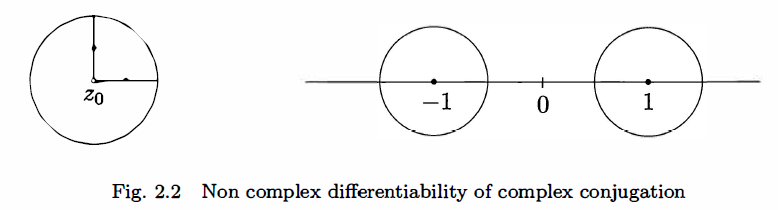
\includegraphics[width=0.8\textwidth]{./SaltChapter/fig-2-2}
\end{center}
\caption{켤레복소수 함수의 미분 불가능성}
\label{fig-2-2}
\end{figure}

$z=z_0+ \dfrac\delta2$로 잡으면, $0<|z-z_0|<\delta$이므로
\begin{equation} \label{eq-2-1}
\left| \dfrac{\bar z - \overline{z_0}}{z-z_0} - g'(z_0) \right| 
= \left| \dfrac{\delta/2}{\delta/2} - g'(z_0) \right| 
= | 1 - g'(z_0)| < \epsilon.
\end{equation}
한편, $z=z_0+ i\dfrac\delta2$로 잡으면, $0<|z-z_0|<\delta$이므로
\begin{equation} \label{eq-2-2}
\left| \dfrac{\bar z - \overline{z_0}}{z-z_0} - g'(z_0) \right| 
= \left| \dfrac{-\delta/2}{\delta/2} - g'(z_0) \right| 
= | 1 + g'(z_0)| < \epsilon.
\end{equation}
식 \eqref{eq-2-1}과 \eqref{eq-2-2}로부터
\[
2 = | 1- g'(z_0) + 1+ g'(z_0)|
\le |1-g'(z_0)| + |1+g'(z_0)| < \epsilon + \epsilon 
= 2\epsilon = 2\cdot\dfrac12 = 1
\]
이 되어 모순이다.
따라서 $g$는 $z_0$에서 복소미분가능하지 않다.
\end{salt_example}

\begin{salt_exercise} \label{ex-2-1}
모든 $z\in\mathbb C$에 대하여 $f(z) = |z|^2$로 정의된
함수 $f:\mathbb C \to \mathbb C$는 $0$에서 복소미분가능하며
$f'(0)=0$임을 보여라.
나중에 (연습문제 \ref{ex-2-9}에서) $f$는 $0$이 아닌 모든 점에서 복소미분 불가능함을 보일 것이다.
\end{salt_exercise}

\begin{salt_exercise} \label{ex-2-2}
영역 $D$에 정의된 함수 $f:D\to \mathbb C$가 복소해석적이라 하자.
$D^* := \{ z\in \mathbb C \,:\, \bar z \in D\}$에 
함수 $f^*:D^* \to \mathbb C$를 $f^*(z) = \overline{f(\bar  z)}$ ($z\in D^*$)로
정의하면 $f^*$가  $D^*$에서 복소해석적임을 증명하라.
\end{salt_exercise}

복소미분 가능성에 대한 다음 변형은 복소미분에 대한 기본 공식을 증명하는 데 유용하게 사용된다.
대략적으로 말하면, 복소미분가능함수 $f$가 $z_0$에서 미분값 $L$을 갖는다면
$f(z)-f(z_0) - L\cdot (z-z_0)$가 $z-z_0$보다 $0$으로 빠르게 수렴함을 뜻한다.

\begin{salt_lemma} \label{lemma-2-1}
$U$가 $\mathbb C$의 열린 집합이고, $z_0\in U$, $f:U\to\mathbb C$라 하면,
다음은 동치이다.
\begin{itemize}
\item[(1)] $f$가 $z_0$에서 복소미분가능하며, $f'(z_0)=L$이다.
\item[(2)] 양수 $r>0$과  $D(z_0,r):=\{z\in\mathbb C\,:\, |z-z_0|<r\}$에 정의된
함수  $h:D(z_0,r)\to \mathbb C$가 존재하여 다음을 만족한다.
\begin{itemize}
\item[(a)] $|z-z_0|<r$에 대하여 $f(z)=f(z_0) + (L+h(z))(z-z_0)$이고,
\item[(b)] $\lim\limits_{z\to z_0} h(z)=0$.
\end{itemize}
\end{itemize}
\end{salt_lemma}

{\bf 증명}

(2)$\Rightarrow$(1):
$z\in D(z_0,r)\setminus \{z_0\}$에 대하여 (a)의 식을 재정리하면,
\[
\dfrac{f(z) - f(z_0)}{z - z_0} - L = h(z) \stackrel{z\to z_0}{\longrightarrow} 0
\]
이므로 $f$는 $z_0$에서 복소미분가능하며 $f'(z_0)=L$이다.

(1)$\Rightarrow$(2):
이제 $f$가 $z_0$에서 복소미분가능하다고 가정하자. 
그러면 $\delta_1>0$이 존재하여 \\
$0<|z-z_0|<\delta_1$, $z\in U$이면 
\[
\left|  \dfrac{f(z) - f(z_0)}{z - z_0}  - f'(z_0) \right| < 1
\]
이다.
$r:=\delta_1$으로 설정하고 함수 $h:D(z_0,r) \to \mathbb C$를 
\[
h(z) = \begin{cases}
\dfrac{f(z) - f(z_0)}{z - z_0} - f'(z_0), & z\ne z_0, \\
0, & z= z_0
\end{cases}
\]
로 정의하자.
그러면 $|z-z_0|<r$일 때
$f(z) = f(z_0) + \left( f'(z_0) + h(z)\right) (z - z_0)$가 성립한다.
이제 (b)를 보이기 위해 $\epsilon>0$이 주어졌다고 하자.
$0<|z-z_0|<\delta$이면
\[
\left|  \dfrac{f(z) - f(z_0)}{z - z_0}  - f'(z_0) \right| \ \left( = |h(z) - 0| \right) < \epsilon
\]
이 되는 $\delta>0$를 잡을 수 있다 ($r$보다 작다는 조건도 만족하도록).
이로써 (a), (b)를 모두 성립함을 알 수 있다. \hfill $\square$

\begin{salt_exercise} \label{ex-2-3}
영역 $D\subset \mathbb C$에 정의된 함수 $f:D\to \mathbb C$가 
$z_0\in D$에서 복소미분가능하다면 $f$는 $z_0$에서 연속임을 보여라.
나중에 우리는 $f$가 $D$에서 복소해석적이면, 
실제로 $D$의 모든 점에서 무한번 미분가능함을 보일 것이다.
\end{salt_exercise}

보조정리 \ref{lemma-2-1}을 이용하여 다음을 쉽게 얻을 수 있다.

\begin{salt_prop}\label{prop-2-1}
$U$가 $\mathbb C$의 열린 부분집합이고,
$f,g: U\to \mathbb C$가 $z_0\in U$에서 복소미분가능함수이면
다음이 성립한다.
\begin{itemize}
\item[(1)] $f+g$는 $z_0$에서 복소미분가능하고
$(f+g)'(z_0) = f'(z_0) = g'(z_0)$이다. \\
(함수 $f+g:U\to\mathbb C$는 $z\in U$에 대하여 $(f+g)(z) = f(z)+g(z)$로 정의한다)
\item[(2)] $\alpha\in\mathbb C$에 대하여 $\alpha\cdot f$는 $z_0$에서 복소미분가능하고
$(\alpha\cdot f)'(z_0) = \alpha f'(z_0)$이다. \\
(함수 $\alpha \cdot f:U\to\mathbb C$는 $z\in U$에 대하여 
$(\alpha \cdot f)(z) = \alpha f(z)$로 정의한다)
\item[(3)] $fg$는 $z_0$에서 복소미분가능하고
$(fg)'(z_0) = f'(z_0)g(z_0) + f(z_0)g'(z_0)$이다.\\
(함수 $fg:U\to\mathbb C$는 $z\in U$에 대하여 
$(fg)(z)= f(z)g(z)$로 정의한다)
\end{itemize}
\end{salt_prop}

\begin{salt_remark}\label{remark-2-1}
$U$가 $\mathbb C$의 열린 부분집합이고,
$\Hol(U)$가 $U$에 정의된 복소해석 함수의 집합이라고 하자.
그러면 위 명제로부터 $\Hol(U)$가 점별 연산에 대하여 복소 벡터공간을 이룸을 알 수 있다.
한편 위 명제의 세번째 내용은 두 복소해석 함수의 점별 곱셈은 다시 복소해석적임을 뜻한다.
따라서 $\Hol(U)$는 점별 덧셈과 곱셈에 대하여
환(ring) 구조를 갖는다.
\end{salt_remark}

\begin{salt_example}\label{example-2-3}
$f(z):=z$ ($z\in \mathbb C$)에 대하여 $f'(z)=1$임을 쉽게 보일 수 있다.
두 복소해석함수의 점별 곱셈에 대한 복소미분 규칙을 이용하면,
수학적 귀납법으로 모든 $n\in \mathbb N$에 $z\mapsto z^n$이 전해석함수이고
\[
\dfrac{d}{dz} z^n = nz^{n-1}
\]
임을 알 수 있다.
특히, 모든 다항식은 전해석함수이다.
\end{salt_example}

\begin{salt_exercise} \label{ex-2-4}
명제 \ref{prop-2-1}을 증명하라.
\end{salt_exercise}


\begin{salt_exercise} \label{ex-2-5}
$\mathbb D = \{ z\in\mathbb C \,:\, |z|<1 \}$이고
$\Hol(\mathbb D)$가 $\mathbb D$에 정의된 복소해석함수의 점별 연산으로 이루어진
복소 벡터공간이라 하자.  $\Hol(\mathbb D)$는 유한차원인가?
\end{salt_exercise}


\begin{salt_exercise} \label{ex-2-6}
$U$가 $\mathbb C$의 열린 부분집합이고,
$U$에 정의된 복소해석함수 $f:U\to \mathbb C$가 
$z\in U$에 대하여 $f(z)\ne 0$라고 하자.
\[
\dfrac 1f : U \to \mathbb C \text{ 를 }
\left( \dfrac 1f \right) (z) = \dfrac 1{f(z)} \text{ 로 정의할 때 }
\]
복소해석함수가 되며 복소미분이 다음과 같음을 보여라.
\[
\left( \dfrac 1f \right)' (z) = - \dfrac{f'(z)}{(f(z))^2} \quad (z\in U).
\]
\end{salt_exercise}

\begin{salt_exercise} \label{ex-2-7}
$\mathbb C\setminus \{0\}$에서 정수 $m\in\mathbb Z$에 대하여
$\dfrac d{dz} z^m = mz^{m-1}$임을 증명하라.
\end{salt_exercise}

실수에서 정의된 합성함수의 미분에 대한 연쇄법식과 같이
복소해석함수의 합성에 대해서도 유사한 연쇄법식이 존재한다.

\begin{salt_prop}[연쇄법칙] \label{prop-2-2} 
\ 
\begin{itemize}
\item[(1)] $D_f$, $D_g$가 복소평면 위의 영역이고,
\item[(2)] $f:D_f \to \mathbb C$가 $D_f$에서 복소해석적이고,
\item[(3)] $g:D_g \to \mathbb C$가 $D_g$에서 복소해석적이고,
\item[(4)] $f(D_f) \subset D_g$일 때,
\end{itemize}
$z\in D_f$에 대하여 $(g\circ f)(z) = g(f(z))$로 정의된
합성함수 $g\circ f : D_f \to \mathbb C$는 $D_f$에서
복소해석함수이고, 
모든 $z\in D_f$에 대하여 $(g\circ f)'(z) = g'(f(z))f'(z)$이다.
\end{salt_prop}

\begin{figure}[!h]
\begin{center}
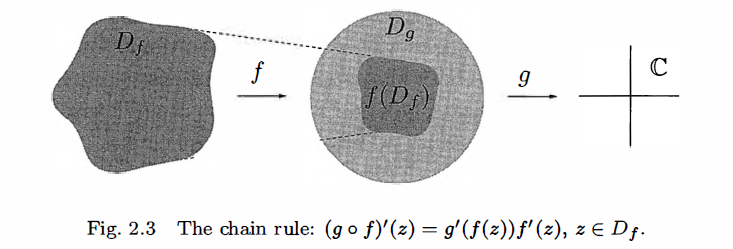
\includegraphics[width=0.7\textwidth]{./SaltChapter/fig-2-3}
\end{center}
\caption{연쇄법칙: $z\in D_f$에 대하여 $(g\circ f)'(z) = g'(f(z))f'(z)$}
\label{fig-2-3}
\end{figure}

{\bf 증명}

$z_0\in D_f$라 하자. 그러면 $f(z_0)\in D_g$이다.
$f$가 $z_0$의 근방에서 복소미분가능하고
$g$가 $f(z_0)$의 근방에서 복소미분가능하므로,
원판 $D(z_0, r_f)\subset D_f$와 $D(f(z_0), r_g) \subset D_g$에 각각 정의된
함수 $h_f$와 $h_g$가 존재하여 다음을 만족한다.
\begin{gather*}
f(z) - f(z_0) = (f'(z_0)+h_f(z))(z-z_0), \\
g(w) - g(f(z_0)) = (g'(f(z_0)) + h_g(w))(w-f(z_0)),
\end{gather*}
또한
\[
\lim_{z\to z_0} h_f(z)=0, \quad
\lim_{w\to f(z_0)} h_g(w)=0.
\]
$f$가 $z_0$에서 연속이므로
$z$가 $z_0$에 가까워질 때 $w:=f(z)$도 $f(z_0)$에 가까워지므로
$z\ne z_0$이고 $z_0$에 가까워지면, 다음 식을 얻는다.
\[
\dfrac{(g\circ f)(z) - (g\circ f)(z_0)}{z-z_0} 
= (g'(f(z_0)) + h_g(f(z)))(f'(z_0) + h_f(z)).
\]
이로써 증명이 끝난다. \hfill $\square$

\begin{salt_example}\label{example-2-4}
연습문제 \ref{ex-2-7}로부터
\[
\dfrac d{dz} \left(\dfrac 1z \right) = - \dfrac 1{z^2}, \quad
z\in \mathbb C \setminus \{0\}
\]
임을 알지만, 복소미분 정의로부터도의 쉽게 유도할 수 있다. 왜냐 하면,
$z_0\in \mathbb C \setminus \{0\}$에 대하여 다음 식이 성립하기 때문이다.
\[
\dfrac{\dfrac 1z - \dfrac1{z_0}}{z-z_0} = \dfrac{z_0 - z}{zz_0(z-z_0)}
= \dfrac{-1}{zz_0} \stackrel{z\to z_0}{\longrightarrow} - \dfrac 1{z_0^2}.
\] 
\begin{figure}[!h]
\begin{center}
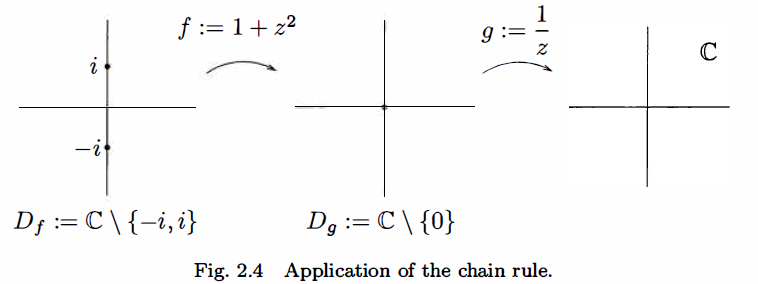
\includegraphics[width=0.7\textwidth]{./SaltChapter/fig-2-4}
\end{center}
\caption{연쇄법칙의 응용}
\label{fig-2-4}
\end{figure}
이제 $D_f:=\mathbb C \setminus \{-i,i\}$에 정의된 함수 $f:= 1+z^2$와
$D_g:=\mathbb C \setminus \{0\}$에 정의된 함수 $g:=1/z$를 생각하자.
$f(D_f) \subset D_g$이 성립함이 명확하므로 연쇄법식에 의해
$\mathbb C \setminus \{-i, i\}$에서
\[
\dfrac d{dz} \left( \dfrac 1{1+z^2} \right) = - \dfrac 1{(1+z^2)^2}\cdot 2z
= - \dfrac{2z}{(1+z^2)^2}.
\]
\end{salt_example}

\begin{salt_exercise} \label{ex-2-8}
$\exp z$가 전해석함수이고 $\exp' z = \exp z$라 가정하고(나중에 증명할 예정이다),
\[
z \mapsto \exp \left( - \dfrac{1+z}{1-z} \right)
\]
가 단위 원판 $\mathbb D := \{ z \in \mathbb C \,:\, |z|<1 \}$에서
복소미분가능함수임을 보이고, 미분을 구하라.
\end{salt_exercise}

\section{코시-리만 방정식}

이제 이 장에서 가장 중요한 결과를 증명해보자.
간략히 말하면, 함수  $f=u+iv$가 복소미분가능하다는 것은
실수부 $u$와 허수부 $v$ ($\mathbb R^2$의 열린 부분집합에 정의된 실함수로 볼 수 있는)가
코시-리만(Cauchy-Riemann) 방정식이라 불리는 편미분 방정식을 만족함과 동치이다. 

\begin{figure*}[!h]
\begin{center}
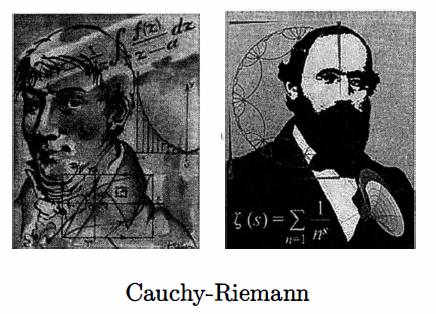
\includegraphics[width=0.4\textwidth]{./SaltChapter/fig-2-0-1} \\
{코시-리만(Cauchy-Riemann)}
\end{center}
%== [salt]?? 캡션을 넣으면 번호가 자동부여?
%\caption{코시-리만(Cauchy-Riemann)}
\end{figure*}


$\mathbb C$의 열린 부분집합 $U$에 정의된
함수 $f:U\to \mathbb C$를 생각하자.
그러면 임의의 점 $(x,y)\in U$에 대하여 $f(x+iy)\in\mathbb C$이고,
$f(x+iy)$의 실수부 $u(x,y)$와 허수부 $v(x,y)$를 그림 \ref{fig-2-5}와 같이 볼 수 있다.

\begin{figure}[!h]
\begin{center}
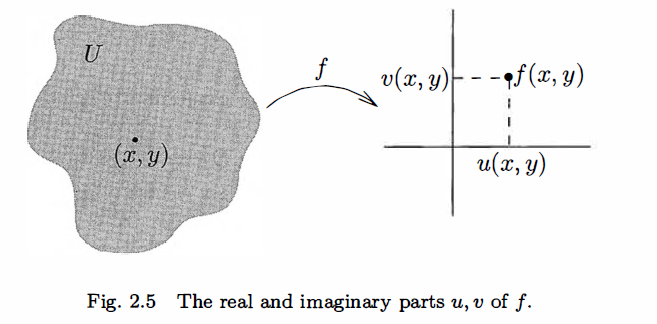
\includegraphics[width=0.6\textwidth]{./SaltChapter/fig-2-5}
\end{center}
\caption{$f$의 실수부 $u$와 허수부 $v$}
\label{fig-2-5}
\end{figure}

점 $(x,y)$가 변하면 $f(x+iy)$도 변하며, $u(x,y)$와 $v(x,y)$도 마찬가지다.
이런 방법으로, $f$와 연관된 실함수를 얻는다.
\begin{align*}
u:U\to \mathbb R, & U \ni (x,y) \mapsto \Re(f(x+iy)) =: u(x,y), \\
v:U\to \mathbb R, & U \ni (x,y) \mapsto \Im(f(x+iy)) =: v(x,y). \\
\end{align*}

이 장의 첫번째 결과는 코시-리만 방정식이 복소미분가능성에 대한 필요조건이라는 것이며
이는 정리 \ref{thm-2-1}에서 증명할 것이다. 
즉, $f$가 $(x_0, y_0) \in U$에서 복소미분가능하다면,

\begin{center}
$(x_0, y_0)$에서
\fbox{
$\dfrac{\partial u}{\partial x} =  \dfrac{\partial v}{\partial y}$ 이고
$\dfrac{\partial u}{\partial y} = - \dfrac{\partial v}{\partial x}$.
}
\end{center}

이를 이 방정식을 코시-리만 방정식이라 부른다.
따라서 복소미분가능함수는 이 방정식을 만족한다.
다시 말하면, 복소함수의 실수부와 허수부가 어떤 점에서 이 방정식을 만족하지 않는다면,
그 점에서 복소미분가능하지 않음을 알 수 있다.
여기서 예제 하나를 보자. 앞에서 우리는 $\epsilon-\delta$를 이용한 복소미분의 정의로부터
직접 계산하여 $z\mapsto \bar z$가 복소평면위의 어느 점에서도 미분가능하지 않음을 보였다.
예제 \ref{example-2-2}를 다시 살펴보자.

\begin{salt_example} \label{example-2-5}
$g(z) = \bar z$ ($z\in \mathbb C$)로 정의된 함수 $g:\mathbb C \to \mathbb C$에 대하여
\begin{align*}
u(x,y) &=\Re(g(x+iy)) = \Re(x-iy) = x, \\
v(x,y) &= \Im(g(x+iy)) = \Im(x-iy) = -y
\end{align*}
이므로
\[
\dfrac{\partial u}{\partial x} = 1 \ne -1 = \dfrac{\partial v}{\partial y}.
\]
이 결과는 코시-리만 방정식이 어떤 점에서도 성립하지 않음을 의미한다.
따라서 $g$가 어떤 점에서도 복소미분가능하지 않다는 이전 결과를 쉽게 얻을 수 있다.
\end{salt_example}


코시-리만 방정식이 복소미분가능성에 대한 필요조건이라는 것을 증명하기에 앞서
이 절에서 증명할 두번째로 중요한 결과로
열린집합에서 복소해석적일 충분조건으로서
코시-리만 방정식에 대하여 언급하고자 한다.
좀 더 정확히 말하면, 
열린집합 $U$에 정의된 함수 $u,v: U\to \mathbb R$가 
$U$에서 연속미분가능하고 (이변수 실함수로서),
$U$의 모든 점에서 코시-리만 방정식을 만족하면,
$u$, $v$로부터 $f(x+iy):=u(x,y) + iv(x,y)$ $(x,y)\in U$로 정의하여 만든
($u$, $v$가 $f$의 실수부와 허수부가 되도록)
새로운 복소함수 $f:U\to\mathbb C$는 복소해석적이다.
이 중요한 결과로부터 우리는
$\epsilon-\delta$ 정의를 이용하는 매우 긴 증명을 통하지 않고
주요 함수의 복소미분가능성을 확인할 수 있다.
예제를 살펴보자.

\begin{salt_example} \label{example-2-6}
뚫린 평면 $\mathbb R^2 \setminus \{(0,0)\}$에서 
\[
u(x,y) := \dfrac{x}{x^2+y^2}, \quad
v(x,y) := \dfrac{-y}{x^2+y^2}, \quad (x,y)\ne(0,0)
\]
로 정의된 함수 
$u$, $v$를 생각하자.
그러면 다음 편미분을 얻는다.
\begin{align*}
\dfrac{\partial u}{\partial x} &= \dfrac{1\cdot(x^2+y^2)-x\cdot 2x}{(x^2+y^2)^2}
= \dfrac{y^2-x^2}{(x^2+y^2)^2}, \\
\dfrac{\partial u}{\partial y} &= \dfrac{-x\cdot 2y}{(x^2+y^2)^2}
= \dfrac{-2xy}{(x^2+y^2)^2}, \\
\dfrac{\partial v}{\partial x} &= \dfrac{2xy}{(x^2+y^2)^2}, \quad
\dfrac{\partial v}{\partial y} = \dfrac{y^2-x^2}{(x^2+y^2)^2}.
\end{align*}
당연히 $\mathbb R^2$에서 $(x,y) \mapsto (x^2+y^2)^2, y^2-x^2, \pm 2xy$는 
연속함수이고, $(x^2+y^2)^2$은 $\mathbb R^2 \setminus \{(0,0)\}$에서 
$0$이 아니다.
따라서 $u$, $v$는 $\mathbb R^2 \setminus \{(0,0)\}$에서 
연속미분가능하다.
또한 코시-리만 방정식이 성립한다. 
결론적으로 $f:=u+iv$는 $\mathbb C\setminus\{0\}$에서 
복소해석적이다.
실제로 위에서 정의한 $f$는 다름 아닌 분수함수 $z\mapsto 1/z$이다.
\[
f=u+iv= \dfrac x{x^2+y^2}+i\left(\dfrac{-y}{x^2+y^2}\right)
= \dfrac{x-iy}{x^2+y^2} = \dfrac{\bar z}{|z|^2} = \dfrac{\bar z}{z \bar z}
= \dfrac  1z, \quad z\ne 0.
\]
\end{salt_example}

\begin{salt_theorem}
$U$가 $\mathbb C$의 열린 부분집합이고
$f:U\to \mathbb C$가 $z_0=x_0+iy_0\in U$에서 복소미분가능하다고 하자.
그러면 함수
\begin{align*}
(x,y) \mapsto u(x,y) & := \Re(f(x+iy)): U\to \mathbb R,
(x,y) \mapsto v(x,y) & := \Im(f(x+iy)): U\to \mathbb R
\end{align*}
는 $(x_0, y_0)$에서 미분가능하고 다음을 만족한다.
\begin{equation} \label{eq-2-3}
\dfrac{\partial u}{\partial x}(x_0,y_0) = \dfrac{\partial v}{\partial y}(x_0,y_0),
\quad
\dfrac{\partial u}{\partial y}(x_0,y_0) = - \dfrac{\partial u}{\partial x}(x_0,y_0),.
\end{equation}
\end{salt_theorem}

{\bf 증명}
(중명의 아이디어는 쉽다. 단지 $(x,y)$를 $(x_0, y_0)$에 가까이 보낼 때
첫번째로 $y$를 $y_0$로 고정하는 방법으로 하고 그 다음에 
$x$를 $x_0$로 고정하는 방법을 사용한 후 각 결과를 살펴본다.
그림 \ref{fig-2-6}을 참고하라.)

\begin{figure}[!h]
\begin{center}
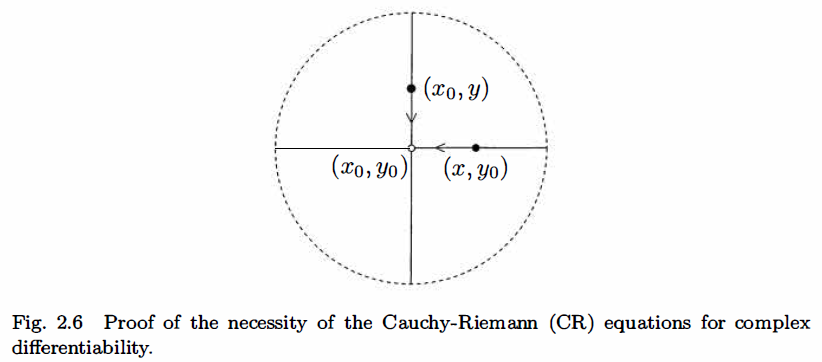
\includegraphics[width=0.9\textwidth]{./SaltChapter/fig-2-6}
\end{center}
\caption{복소미분가능성에 대하여 코시-리만(CR) 방정식이 필요조건임을 증명}
\label{fig-2-6}
\end{figure}

$z_0 = (x_0, y_0)\in U$라 하자.
$\epsilon>0$에 대하여, 
$0<|z-z_0|<\delta$일 때 $z\in U$에 대하여
\begin{equation}\label{eq-2-4}
\left| \dfrac{f(z)-f(z_0)}{z-z_0} - f'(z_0) \right| < \epsilon
\end{equation}
을 만족하는 $\delta >0$가 존재한다.

{\bf 단계 1:}
$\dfrac{\partial u}{\partial x}(x_0,y_0)$가 존재하고 $\Re(f'(z_0))$와 같음을 보인다.















